% \documentclass{report}
% 
% \usepackage{fancyhdr}
\usepackage{fourier-orns}
\usepackage{hyperref}%% To refrence links / jumps
\usepackage{chngcntr} %% For some extra counters numberings
\usepackage[a4paper, right = 0.5in, left = 0.5in,top = 1in , bottom = 1in]{geometry}
\usepackage{etoolbox} %% Provides like a language for advanced customization
\usepackage{datetime} %% For dates of course
\usepackage{lastpage} %% provides pages numbers
\usepackage[sc]{titlesec} %% modify titles
\usepackage{enumerate}
\usepackage{cancel}
\usepackage{tikzsymbols}
\usepackage[dvipsnames]{xcolor}
\usepackage{import}
\usepackage{pdfpages} %% include other pdfs
\usepackage{transparent} %% Transparency
\usepackage{xcolor}  %% Colors
\usepackage[many]{tcolorbox}
\usepackage[framemethod=TikZ]{mdframed}
\usepackage{amsmath,amsfonts,amsthm,amssymb,mathtools}
\usepackage{tikz}
\usepackage{bookmark}
\usepackage{graphicx}
\usepackage{mathpazo}

\usepackage{fontawesome5}

\linespread{1.5}


\titleformat{\chapter}[display]   
{\fontfamily{ppl}\selectfont\huge\color{YellowOrange!80!orange}} % Font style and size 
{\raggedleft\color{purple}\fontsize{70}{0pt}\selectfont\thechapter}   
{-1.5cm}    			                          % Space between the chapter number and title
{
	\begin{tikzpicture}[overlay]
		\node[anchor = west,yshift = 0.2cm,xshift = -1cm] {\fontsize{90}{20} $\int_{}^{} $};
		\node[yshift = 4cm, xshift = 17cm]   {\includegraphics[width = 4cm]{preview0}};
	\end{tikzpicture}
\hspace{1cm}\Huge\raggedright\MakeUppercase}

\titleformat{\section}[block]
{
\fontfamily{ppl}\selectfont\huge\color{YellowOrange!80!orange}
}
{
\color{purple}\fontsize{20}{0pt}\selectfont\thesection 
}
{0cm}
{
	\begin{tikzpicture}[overlay]
		\node[anchor = west,yshift = 0.2cm,xshift = -0.4cm, circle = 1pt] {};
	\end{tikzpicture}
}

\titlespacing*{\section}{0pt}{0.7cm}{1.5cm}


\newcommand{\divider}
{
	\begin{center}
	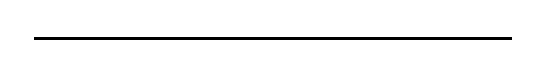
\begin{tikzpicture}
		\draw[thick, black] (0.25*\textwidth, 0) -- (0.75*\textwidth, 0);
		\node[rotate = 360 - 90, xshift = -0.6pt, yshift = 1pt] at (0.25*\textwidth,0){\decotwo};
		\node[rotate = 90, xshift = -0.6pt, yshift = 1pt] at (0.75*\textwidth,0){\decotwo};
	\end{tikzpicture}
	\end{center}
}

\pagestyle{fancy}

\newcommand{\lecday}[1][]
{
    \def\datee{#1}
    \fancyhead[L]{\datee}
}



\newcommand{\signature}
{
	\begin{tikzpicture}[remember picture,overlay]
		\node[fill = YellowOrange!20!white] at ([yshift = 1cm, xshift = -3cm]current page.south east) {\fontsize{10pt}{0pt}{\itshape Kara.$\mathcal{A}$}};
	\end{tikzpicture}
}

\AddToHook{shipout/background}{
  \begin{tikzpicture}[remember picture, overlay]
	  \node[] at ([yshift = 1.5cm,xshift = \textwidth /2 + 0.9cm]current page.south west) {\includegraphics[width = 0.5cm]{preview3}};
	  \node[] at ([yshift = 1.5cm,xshift = - \textwidth /2 - 0.9cm]current page.south east) {\includegraphics[width = 0.5cm]{preview4}};
  \end{tikzpicture}
}



\newtcolorbox[auto counter, number within = section]{remark}[1][]
{
       		title = Remark #1,
		enhanced,
		boxrule = 0pt,
		colback = white,
		breakable,
		arc = 4pt,
		colbacktitle = cyan,
		colback = cyan!5!white,
		segmentation style =
		{
			solid,cyan,thick,
		},
		attach boxed title to top left =
		{
			xshift = 0cm,
		},
		boxed title style =
		{
			boxrule = 0pt,
			sharp corners,
			drop fuzzy shadow = {cyan},
		},
		drop fuzzy shadow = {cyan!80!black},
}

\newtcolorbox[auto counter, number within = section]{theorem}[1][]
{                                      
		title = Theorem \thetcbcounter : #1,
		enhanced, 
		boxrule = 0pt,
		colback = white,
		breakable,
		arc = 4pt,
		colbacktitle = purple,
		colback = purple!5!white,
		segmentation style = 
		{
			solid, purple,thick,
		},
		attach boxed title to top left = 
		{
			xshift = 0cm, 
		},
		boxed title style = 
		{
			boxrule = 0pt,
			sharp corners,
			drop fuzzy shadow = {purple},
		},
		drop fuzzy shadow = {purple!80!black},
}

\newtcolorbox[auto counter, number within = section]{definition}[1][]
{                                      
		title = Definition \thetcbcounter : #1,
		enhanced, 
		boxrule = 0pt,
		colback = white,
		arc = 4pt,
		breakable,
		colbacktitle = YellowOrange!80!black,
		segmentation style = 
		{
			solid, YellowOrange,thick,
		},
		attach boxed title to top left = 
		{
			xshift = 0cm, 
		},
		colback = YellowOrange!5!white,
		boxed title style = 
		{
			boxrule = 0pt,
			sharp corners,
			drop fuzzy shadow = {YellowOrange!80!orange},
		},
		drop fuzzy shadow = {YellowOrange!80!black},
}

\newtcolorbox[auto counter, number within = section]{corollary}[1][]
{                                      
		title = corollary \thetcbcounter : #1,
		enhanced, 
		boxrule = 0pt,
		colback = white,
		arc = 4pt,
		breakable,
		colbacktitle = YellowOrange!80!black,
		segmentation style = 
		{
			solid, YellowOrange,thick,
		},
		attach boxed title to top left = 
		{
			xshift = 0cm, 
		},
		colback = YellowOrange!5!white,
		boxed title style = 
		{
			boxrule = 0pt,
			sharp corners,
			drop fuzzy shadow = {YellowOrange!80!orange},
		},
		drop fuzzy shadow = {YellowOrange!80!black},
}


\newtcolorbox{example}[1][]
{                                      
		title = Example,
		enhanced, 
		boxrule = 0pt,
		colback = white,
		arc = 4pt,
		segmentation style = 
		{
			solid, SpringGreen,thick,
		},
		breakable,
		colback = SpringGreen!5!white,
		colbacktitle = SpringGreen!80!black,
		attach boxed title to top left = 
		{
			xshift = 0cm, 
		},
		boxed title style = 
		{
			boxrule = 0pt,
			sharp corners,
			drop fuzzy shadow = {SpringGreen!80!orange},
		},
		drop fuzzy shadow = {SpringGreen!80!black},
}


\newcommand{\integral}[4]{\int\limits_{#1}^{#2} #4 d#3}
\newcommand{\limit}[3]{\lim\limits_{#1 \rightarrow #2} #3}
\newcommand{\strone}[2]{\left[ \begin{gathered}#1\\ #2\end{gathered} \right] }
\newcommand{\strtwo}[2]{\left\{ \begin{gathered}#1\\ #2\end{gathered} \right\} }
\newcommand{\strthree}[2]{\left\lfloor \begin{gathered}#1\\ #2\end{gathered} \right\rfloor }


\newcommand{\startbf}[1]{\text{\bfseries{#1}}}
\newcommand{\sett}[1]{\left\{ #1 \right\}}
\newcommand{\thesis}[1]{\left( #1 \right)}
\newcommand{\brkt}[1]{\left[ #1 \right]}
\newcommand{\floor}[1]{\left\lfloor #1 \right\rfloor}


\DeclareMathOperator{\img}{im} % Image
\DeclareMathOperator{\Img}{Im} % Image
\DeclareMathOperator{\coker}{coker} % Cokernel
\DeclareMathOperator{\Coker}{Coker} % Cokernel
\DeclareMathOperator{\Ker}{Ker} % Kernel
\DeclareMathOperator{\rank}{rank}
\DeclareMathOperator{\Spec}{Spec} % spectrum
\DeclareMathOperator{\Tr}{Tr} % trace
\DeclareMathOperator{\pr}{pr} % projection
\DeclareMathOperator{\ext}{ext} % extension
\DeclareMathOperator{\pred}{pred} % predecessor
\DeclareMathOperator{\dom}{dom} % domain
\DeclareMathOperator{\ran}{ran} % range
\DeclareMathOperator{\Hom}{Hom} % homomorphism
\DeclareMathOperator{\Mor}{Mor} % morphisms
\DeclareMathOperator{\End}{End} % endomorphism


\newcommand{\lm}{\ensuremath{\lambda}}
\newcommand{\eps}{\ensuremath{\epsilon}}
\newcommand{\veps}{\ensuremath{\varepsilon}}
\newcommand{\al}{\ensuremath{\alpha}}
\newcommand{\bb}{\ensuremath{\beta}}
\newcommand{\cc}{\ensuremath{\gamma}}
\newcommand{\dd}{\ensuremath{\delta}}
\newcommand{\DD}{\ensuremath{\Delta}}
\newcommand{\ff}{\ensuremath{\phi}}
\newcommand{\FF}{\ensuremath{\varphi}}

\newcommand{\RR}{\mathbb{R}}
\newcommand{\RO}{\mathcal{R}}
\newcommand{\EE}{\mathbb{E}}
\newcommand{\CC}{\mathbb{C}}
\newcommand{\RW}{\mathbb{R}^2}
\newcommand{\RT}{\mathbb{R}^3}
\newcommand{\RN}{\mathbb{R}^n}
\newcommand{\DS}{\mathcal{D}}

\newcommand{\KK}{\mathbb{K}}
\newcommand{\KW}{\mathbb{K}^2}
\newcommand{\KT}{\mathbb{K}^3}
\newcommand{\KN}{\mathbb{K}^n}

\newcommand{\NN}{\mathbb{N}}

\newcommand{\PS}{\mathcal{P}}
\newcommand{\AS}{\mathcal{E}}
\newcommand{\FS}{\mathcal{F}}
\newcommand{\LS}{\mathcal{L}}
\newcommand{\MS}{\mathcal{M}}

















% 
\lecday[2025-05-27]

% \begin{document}

\section{The Hilbert Projection Theorem}

\begin{theorem}[(Hilbert)]
  Let $H $ be a Hilbert space and $C $ be
  a non empty subset of $H $ which is closed and 
  convex, Then forevery $x \in  H $, there exits
  a unique $u \in  C $, such that : 
  \[
  \| x-u \| =
  d(x,C) \quad \quad \quad (1) 
  \]
  in addition, $u $ is characterized by 
  the property : 
  \[
    \begin{cases}
       u \in  C  \\
      \mathcal{R} \left\langle x-u, v-u \right\rangle  
      \leq  0 \quad \quad  \forall  v \in  C \quad 
      \quad \quad \quad \quad \quad 
      (2) 
    \end{cases}
  \]
\end{theorem}

\begin{proof}
let $x \in  H$ be fixed. By definition 
of $d(x,C)$ which is : 
\[
d(x,C)  := \inf_{u \in  C} \| x-u \| 
\]
there exists for all $n \in \NN$, a vector 
$u_{n} \in C $  such that : 
\[
d(x, C)  \leq 
\| x - u_{n} \|  <  
d(x, C)  + \frac{1}{n} \quad \quad 
\quad (*) 
\]
Let us show that $(u_{n}) _{n \in  \NN} $  is 
Cauchy. \\
For all $p,q \in \NN $, we have : 
\begin{align*}
\| u_{p} - u_{q} \|  ^2  
&= 
\| (x- u_{p}) - (x-u_{q})  \|  ^2  
\\
&\overset{ \textcolor{red}{P.I}}{=}     
2 \left( 
  \| x-u_{p} \| ^2  + 
  \| x-u_{q} \|  ^2  
\right) - 4 
\| x - \frac{u_{p} + u_{q}}{2} \|  ^2 
\end{align*}
Next by $(*)$, we have : 
\begin{align*}
  \| x - u_{p} \|  & < 
  d(x, C) + \frac{1}{p} \\
  \| x-u_{q} \| & <  
  d(x, C)  + \frac{1}{q}
\end{align*}
On the other hand, since $C $ 
is convex and $u_{p}, u_{q} \in  C $, then 
$\frac{u_{p} + u_{q}}{2} \in C $. Thus : 
\[
\| x-  \frac{u_{p} + u_{q}}{2} \|  
\geq d(x,C) 
\]
hence : 
\[
\| u_{p} - u_{q} \| ^2  
\leq 2 \left( 
  (d(x,C) + \frac{1}{p}) ^2  + 
  (d(x, C) + \frac{1}{q}) ^2 
\right) - 4 d(x,C) ^2  \rightarrow  0
\quad \quad \quad 
p,q \rightarrow +\infty 
\]
hence we have : 
\[
\| u_{p} - u_{q} \|  \rightarrow 0 \quad 
\quad \quad 
p,q \rightarrow + \infty 
\]
Showing that $(u_{n}) _{n \in \NN} $ is a 
Cauchy sequence of $H$. since $H $ is complete
then $(u_{n}) _{n \in \NN} $  
is convergent to some $u \in  H $. Next, 
since $(u_{n}) _{n \in \NN} \in C $ and $C $ 
is closed then $u \in  \overline{C} = C $. Therefore
$u \in  C$, thus by setting 
$n \rightarrow \infty  $ in $(*)$. we get : 
\[
\| x-u \| = d(x,C) 
\]
The existence of $u $ is proved.  \\ 
\underline{
The uniqueness of $u $ :
}
Let $u, u'  \in C $ such that : 
\[
\| x-u \|  = \| x-u' \|  = 
d(x,C) 
\]
then we have : 
\begin{align*}
  \| u-u' \|^2   &= 
\| (x-u) -(x-u') \| ^2  
\\
                 & \overset{\textcolor{red}{P.I}}{=}  
              2 \left( 
                \| x-u \| ^2  + 
                \| x-u' \| ^2 
              \right) - 
              4 \| x-
              \underbrace{
              \frac{u + u'}{2} 
              }_{ \in  C \text{ (convex) } } 
              \| ^2  \quad  \quad  \quad  (*) 
\end{align*}
Thus : 
\[
\| x- \frac{u + u'}{2} \|  
\geq d(x,C) 
\]
from $(*)$ we continue : 
\[
 (*) \leq  
 2 \left( 
   d(x,C) ^2  + 
   d(x,C) ^2 
 \right)- 4 
 d(x,C) ^2  = 0
\]
Thus $\| u-u' \| = 0$, implying that 
$u = u' $. Hence the uniqueness of $u $ is proved. 
\\
\textsc{The equivallence between $(1)  $ and $(2)  $ :}
\\
\[
  (1)  \implies (2) 
\]
Let $u \in  C $, satisfyin $(1)$ i.e. $(\| x-u \| = d(x,C) )  $ and 
show that $(2)$ i.e. $(\forall v \in  C : 
\mathcal{R} \left\langle x-u, v-u \right\rangle \leq 0)$. for every 
$v \in  C $, consider the vectors $w_{t} (t \in  [0,1])  $, defined by : 
\[
w_{t} := 
(1-t) u + t v
\]
Since $C $ is convex then $w_{t} \in C $, then we have 
\[
  \| x-w_{t} \|  \geq  d(x, C) = \| x-u \|  \quad 
  \left( \forall  t \in  [0,1] \right)
\]
That is : 
\[
\| x - (1-t)u - tv  \|  
\geq \| x-u \|  \quad \left( \forall  t \in [0,1] \right)
\]
That is : 
\[
\|(x-u) - t(v-u)  \|  \geq 
\| x-u \|  \quad \left( 
  \forall t \in  [0,1]
\right)
\]
By squaring, we get : \footnote{
  $\| a-b \| ^2  = \| a \| ^2  + \| b \| ^2  - 
  2 \mathcal{R} \left\langle a,b \right\rangle $ 
}
\begin{align*}
\cancelto{}{
\| x-u \| ^2 
} 
+ 
\| v-u \| ^2 t ^2 
- 2 t \mathcal{R} 
\left\langle x -u, v -u \right\rangle  
\geq 
\cancelto{}{
\| x-u \| ^2 
}  \quad \quad \quad 
\left( \forall t \in  [0,1] \right)
\end{align*}
hence : 
\[
\| v-u \| ^2  t - 2 \mathcal{R} 
\left\langle 
  x-u, v-u
\right\rangle  \geq 0 \quad 
\quad \left( 
  \forall  t \in  (0,1]
\right)
\]
i.e. 
\[
\mathcal{R} \left\langle 
  x-u, v-u
\right\rangle  \leq 
\frac{t}{2}
\| v-u \| ^2  \quad \quad 
\left( 
  \forall t \in (0,1]
\right)
\]
now setting $t \rightarrow^{>} 0 $, we get finally : 
\[
\mathcal{R} \left\langle 
  x-u, v-u
\right\rangle  \leq 0
\]
as required. 
\[
(2)  \implies (1)   
\]
Conversely, let $u \in  C $ satisfying $(2)$ 
\[
  \mathcal{R} \left\langle x-u, v-u \right\rangle  \leq 0 \quad 
  \quad \left( \forall v \in  C \right)
\]
and let us show that $u $ satisfies $(1)$ i.e. 
\[
\| x-u \|  = d(x,C)  
\]
for all $v \in  C $, we have : 
\begin{align*}
\| x-u \| ^2  - 
\| x-v \| ^2  &= 
\| x-u \| ^2  - 
\| (x-u)  -(v-u)  \| ^2  
\\
&= 
\| x-u \| ^2  - 
\left( 
  \| x-u \| ^2  
  + \| v-u \| ^2  
  - 2 \mathcal{R} 
  \left\langle x-u, v-u \right\rangle 
\right) 
\\
&=
2 \mathcal{R} 
\left\langle 
  x-u, v-u
\right\rangle  - 
\| v-u \| ^2 
\leq  0
\end{align*} 
that is : 
\[
\| x-u \| \leq 
\| x-v \|  \quad 
\left( 
  \forall  v \in  C
\right)
\]
By taking the infimum on $v \in C $, we get :
\[
\| x-u \|  
\leq d(x,C) 
\]
Hence 
\[
\| x-u \| = d(x,C) 
\] 
Hence. 
\[
\| x-u \| = d(x,C) 
\]
As required. This completes the proof.
\end{proof}

\begin{definition}[]
Let $H $ be a hilbert space and 
$C $ be a non empty subset of $H$. 
Which is closed and convex. 
The map associating to each $x \in  H $
the unique $u \in  C $ such that. 
\[
\| x-u \| = d(x,C) 
\]
is called "The projection on $C $ " and we denote
it by $\pi _{C} $ \footnote {
  \it Notice $d(\pi (x) , \pi (y) ) 
  \leq d(x,y) $ }
\end{definition}
\begin{theorem}[]
Let $H $ be a Hilbert Space and 
$C $ be a non empty subset of $H $ 
which is closed and convex. Then the map
$\pi _{C} $ is $1 $-Lipschitz (so continuous).
\end{theorem}
\begin{proof}
For $x,y \in  H $, let $ u := 
\pi _{C}(x) $ and $v := \pi _{C}(y)  $. 
So we have to show that : 
\[
\| u-v \|  
\leq \| x-y \| 
\]
Since this inequality is trivial when $u=v $. 
we may suppose that $u \neq v $. According to the 
second part of the theorem $1 $, we have that : 
\[
\mathcal{R} \left\langle x-u, v-u \right\rangle  
\leq 0 \quad 
\quad 
\quad (A) 
\]
and 
\[
\mathcal{R} 
\left\langle 
  y-v, u-v
\right\rangle  
\leq 0
\]
that is : 
\[
\mathcal{R} 
\left\langle 
  v-y, v-u
\right\rangle  
\leq 0  \quad \quad \quad 
(B) 
\]
Summing sides to side $(A) $ and 
$(B)$, we get : 
\[
\mathcal{R}  
\left\langle 
  (x-u) + (v-y), 
  v-u
\right\rangle  
\leq 0
\]
i.e. 
\[
\mathcal{R} \left\langle 
  (x-y) + (v-u), v-u 
\right\rangle  \leq 0
\]
that is : 
\[
  \mathcal{R} 
  \left\langle 
    x-y, v-u
  \right\rangle  + 
  \| v-u \| ^2  \leq  0
\]
Thus : 
\begin{align*}
\| v-u \| ^2 
& \leq 
- \mathcal{R} \left\langle 
  x-y, v-u
\right\rangle  \\
& \leq 
\left| 
\left\langle x-y, v-u \right\rangle 
\right| \\
& \leq^{C.S} 
 \| x-y \| \cdot 
 \| v-u \| 
\end{align*}
Hence : 
\[
\| v-u \|  
\leq \| x - y \| 
\]
as required.
\end{proof}
\begin{corollary}[]
Let $H $ be a Hilbert space and $K $ be 
a closed vector subspace of $H $. For all 
$x \in  H$, the projection $u = \pi _{K}(x)  $   
of $x $ on $K $ is characterized by : 
\[
  u \in  K \\
  \left\langle 
    x-u, v
  \right\rangle=
   0 , \quad \forall  v \in  K
\]
In addition $\pi _{K} \in 
\mathcal{L} (H)$ (i.e. $\pi _{K} $ 
is linear and continuous).
\end{corollary}
\begin{proof}
$(\KK = \CC )$ i.e. in the general case. \\ 
let $x \in  H$ and $u := \pi _{K}{x} $ 
by the second part of Theorem $1$, $u $ 
is characterized by : 
\[
  \begin{cases}
    u \in  K \\`
    \mathcal{R} \left\langle 
      x-u, w-u
    \right\rangle  \leq 0 \quad  \quad \quad 
    \left( \forall w \in  K\right) 
    \quad  \quad \quad (I) 
  \end{cases}
\]
since $K $ is vector subspace of $H $ then 
any vector $w \in  K $. Can be written 
as 
\[
w = z v + u \quad \quad \left( 
  z \in  \CC , \quad v \in K
\right)
\]
and conversly any vector fof the form 
$zv + u, \quad (z \in  \CC, \quad v \in K) $ belong 
to $K $. Thus $(I)$ is equivalent to : 
\[
\mathcal{R} \left\langle 
  x-u, zv
\right\rangle  \leq 0 \quad \left( 
  \forall  z \in \CC , \quad  \forall v \in  K
\right)
\]
That is : 
\[
\mathcal{R} 
z
\left\langle 
  x-u, 
  v
\right\rangle  \leq 0 \quad \left( 
  \forall z \in  \CC , \quad 
  \forall v \in  K
\right) \quad \quad \quad 
(II) 
\]
for $(II)$ to be satisfied for all 
$z \in  \CC$, 
it suffices that it tobe satisfied
for all $z$ real and 
all $z $ pure imaginary. \\
For $z $ real say $z = t \in \RR  $, we get : 
\[
t \mathcal{R} \left\langle 
  x-u, v
\right\rangle  \leq 0 \quad \quad 
\left( 
  \forall  t \in  \RR ,
  \forall  v \in  K
\right)
\]
which is equivalent to : 
\[
\mathcal{R} \left\langle 
  x-u, v
\right\rangle  = 0 \quad \quad 
\left( 
  \forall  v \in  K
\right)
\]
for $z $ pure imaginary, say $z = 
it, \quad t \in \RR $. We get : 
\[
  \mathcal{R} 
  it \left\langle 
    x-u, v
  \right\rangle  \leq 0 \quad 
  \quad 
  \left( 
    \forall t \in \RR , \quad 
    v \in  K
  \right)
\]
\footnote{
  \[
  \mathcal{R}(iz)   = - \mathcal{I}  (Z) 
  \]
}
which is equivalent to 
\[
\mathcal{I} 
\left\langle 
  x-u, v
\right\rangle  = 0 \quad 
\quad \left( 
  \forall v \in  K
\right) \quad \quad (2) 
\]
So : 
\[
  (II)  \iff (1)  \quad \&  \quad (2) 
\]
\[
\iff \left\langle x-u, v \right\rangle  
= 0 \quad \quad 
\left( 
  \forall v \in  K
\right)
\]
This proves the first point of
the corollary . 
Further, the continuity of $\pi _{K} $ 
is proved in Proposition $2 $. So, it remains
to show the linearity of $\pi _{K} $. 
let $x,y \in  H $ and $\lm,\mu \in  \CC  $ and 
let us show that 
\[
\pi _{K}(\lm x + \mu  y)  
= 
\lm \pi _{K}(x)  + 
\mu \pi _{K}(y) 
\]
we have for all $v \in K $ :
\begin{align*}
\left\langle 
  \lm x + \mu  y- 
  (\lm \pi _{K}(x) + \mu \pi _{K}(y) ) , v
\right\rangle &=
\left\langle 
  \lm(x - \pi _{K}(x) )  + 
  \mu (y - \pi _{K}(y) )  , v
\right\rangle  \\
              &= 
             \overline{\lm} 
           \left\langle 
             x - \pi _{K}(x), v 
           \right\rangle  + 
           \overline{\mu }
           \left\langle 
             y - \pi _{K}(y) , v
           \right\rangle       \\
              &= 0
\end{align*}
Thus. 
\[
\left\langle 
  \lm x + \mu  y - 
  (\lm \pi _{K}(x) + \mu \pi _{K}(y)  ), v
\right\rangle  = 0 
\quad \left( 
  \forall  v \in  K
\right)
\]
implying by the result of the first part, that: 
\[
\pi _{K}(\lm x + \mu y)  =
\lm \pi _{K}(x)  + \mu \pi _{K}(y) 
\]
Show that $\pi _{K} $ is linear. This completes
the proof.
\end{proof}
\begin{corollary}[]
Let $H $ be a hilbert space and $K $ 
be a closed vector subspace
of $H $. \\
Then $K^{\bot } $, closed vector subspace 
of $H $ ænd it s a complement subspace
of $K$ in $H $ i.e. 
\[
K \oplus K = H
\]

\end{corollary}
% \end{document}
